	\appendix
	\section{Invertible Transformation and Tolerance Testing}
	
	In the last section, we shrink the data vector and covariance matrices and find the most cosmological-informative modes in both. However, in order to make a tolerance testing of each element in the covariance, we not only need the cosmological-informative modes but also the uninformative modes. Suppose we find the informative set of modes for cosmology, the modes that are orthogonal to them, or the complementary set of the informative one, form a set of modes that are cosmological-uninformative. 
	
	To find these modes, we start off with the compression scheme presented in Eq. \ref{eq:compression_scheme}, which will serve as the basis for a rotation matrix $W_\alpha$. We then use the Gram-Schmidt decomposition to create $227 - N_p$ vectors orthonormal to $U_{\alpha}$, thus obtaining a unitary $227 \times 227$ matrix. We then have,
	\be
	C'_{\alpha\beta} = W_{\alpha i} C_{ij} W^T_{j\beta}.
	\ee
	%When this transformation is applied to the original matrix, $C_{ij}$, the first $N_p \times N_p$ elements of the new matrix will be the same as we had in $C_{\alpha\beta}$. Since our transformation spreads out the information contained in the compressed matrix, the relevant values for parameter estimation will be contained in the first $N_p$ rows and columns of the new covariance matrix. This means that we will have $N_p \left( 2 \times 227 - N_p \right)$ important elements, which is about an order of magnitude less than in the case of the full covariance matrix.
	
	\begin{figure}[]
		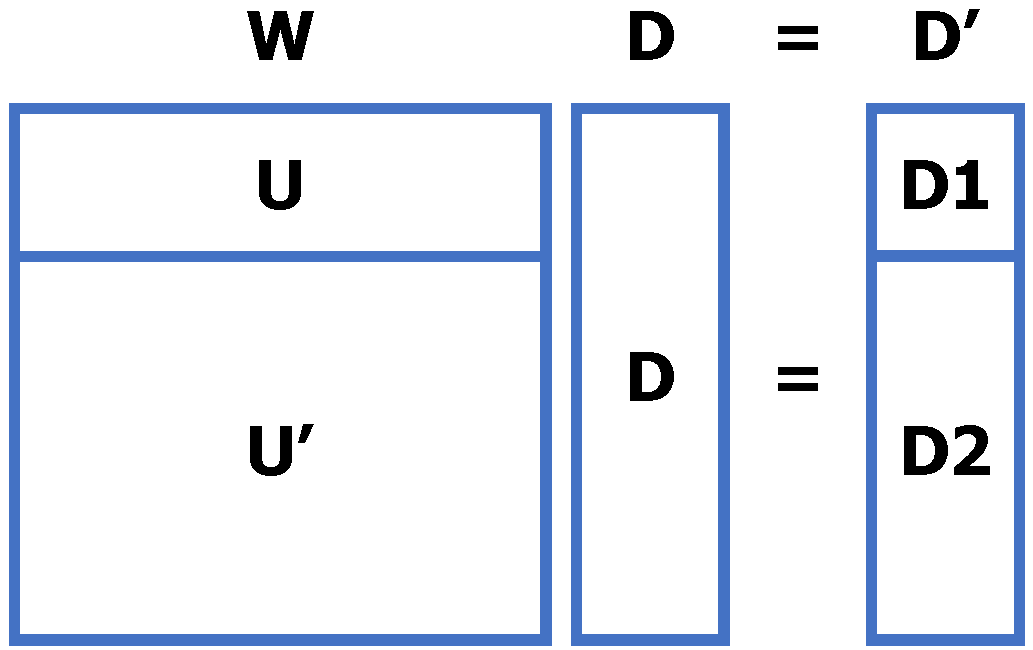
\includegraphics[width=0.45\columnwidth]{Transformation_data.pdf}
		
		\bigskip
		
		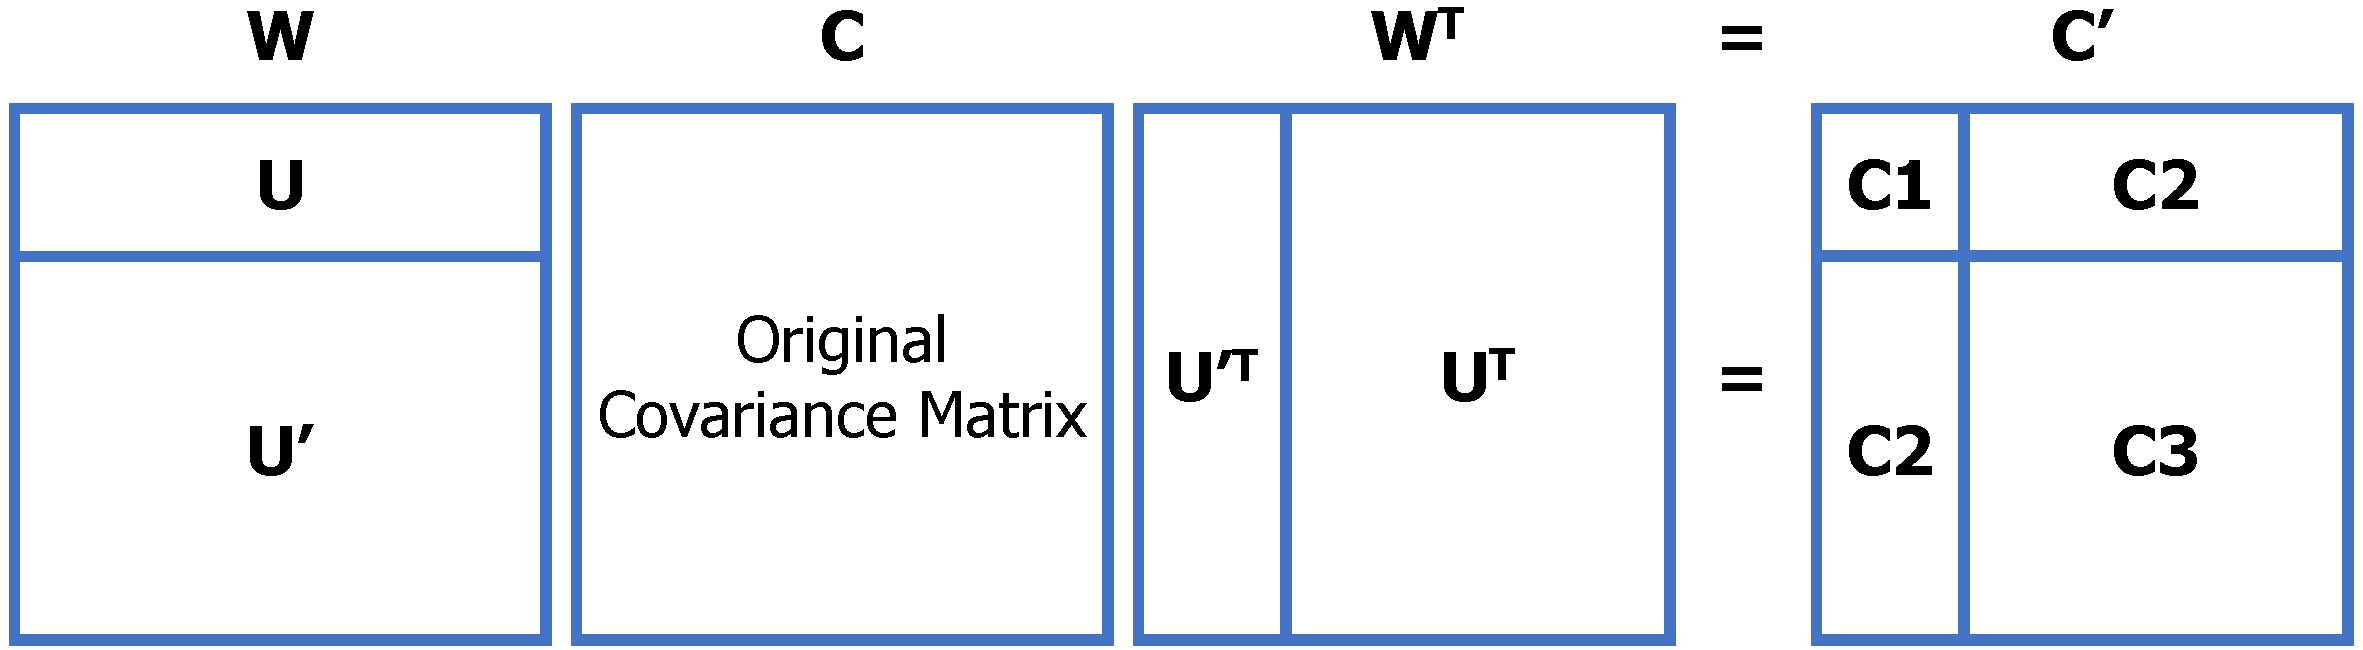
\includegraphics[width=0.99\columnwidth]{Transformation_CM.pdf}
		\caption{Illustration of the invertible transformation, $W$. It's components, $U$ and $U'$ are the compression scheme described in Sections \ref{subsec:shrinkage} and orthogonal components obtained using the Gram-Schmidt decomposition, respectively. \textbf{Top:} Transformation of the data vector, where D1 corresponds to compressed set, and D2 are uninformative for parameter constraints. \textbf{Bottom:} Transformation of the covariance matrix. The last square on the right, $C'$ is divided into four blocks: C1 is the most informative to cosmology, C2 are also relevant to constraints, but on a lower scale, and, finally, C3 is irrelevant to the $\chi^2$ calculation. \label{fig:transformation}}
	\end{figure}
	
	With the invertible transformation $W$, shown in \figref{transformation}, the data vector and covariance matrix are transformed into sectional blocks. We will describe the meaning of each block here. The data vector is split into two blocks: D1 has the transformed data points that are sensitive to changes in the cosmological parameters, that is, the cosmological-sensitive data; D2 is generated by the modes that are orthogonal to D1, they will, in principle, be unaffected by changes to the cosmological parameters, which makes them uninformative for parameter constraints.
	
	The transformed covariance matrix is split into 4 blocks, with the off-diagonal ones being the transpose of each other. Block C1 is the variance and covariance of the cosmological-sensitive data, D1, it describes how well the cosmological-sensitive data is measured, and is, therefore, the one that contributes most to the $\chi^2$ calculation, and, consequently, to parameter constraints. Block C2 is the cross-correlation between D1 and D2, it is important for parameter constraints because it describe how D1 is affected by the uncertainty of D2.  Finally, C3 relates to the uninformative data, D2; it plays a minor role to $\chi^2$, so it affects the parameter constraints least.
	
	%With this invertible transformation W shown in \figref{illu-trans}, the data vector and covariance matrix are transformed into sectional blocks. We will describe the meaning of each blocks here. The data vector is split into two blocks. D1 is the block of transformed data points that are sensitive to the changes in cosmological parameter set, that is, the cosmological-sensitive data. D2 is generated by the modes that are orthogonal to the cosmological sensitive mode, they will in principle stays relatively constant when cosmological parameter changes and are uninformative for parameter constraints.
	
	%The transformed covariance matrix is split into 4 blocks, with the off-diagonal blocks being the transpose of each other, there are 3 different blocks. Block C1 is the variance and covariance of the cosmological informative data, or D1. This block contributes almost everything to the $\chi^2$ calculation. C1 describes how well the cosmological-sensitive data is measured, so the value in this block will affect the parameter constraints. Block C2 is the variance and covariance of the uninformative data, or D2. It plays a minor role in the $\chi^2$, so it will affect the parameter constraints less. C3 is the cross-correlation between D1 and D2, and it will affect the parameter constraints because it describes how D1 is affected by the uncertainty of D2.
	
	The next step is then to test the tolerance of different parts of the transformed covariance matrix. We first compare the results of increasing the error of each block separately by a factor of 100 and compare the results to constraints with the unmodified covariance, then we start by introducing smaller errors to the relevant blocks, C1 and C2 and analyse the corresponding increase in the parameter constraints.
	
	\section{Tolerance Testing}
	
	Given that block C1 contains the same elements as those in the compressed covariance matrix, it is intuitive to think that this is the only block relevant for parameter constraints. It is clear, however, in 	\figref{tolerance1000} that this is not the case. Multiplying the elements of blocks C1 and C3 do not alter the constraints, whereas changes made to blocks C2 and C1+C2 do. To explain this, we need to look at what happens to $\chi^2$ when using the transformed data set and covariance matrix. We have
	\be
	\chi^2 = \mathbf{(D - T)\ C^{-1}\ (D-T)}^t
	, \ee
	where $\mathbf{C}^{-1}$ is the inverse of the covariance matrix, $\mathbf{D}$ is the data set and $\mathbf{T}$ is the theory prediction (in our case, for $\xi_+$ and $\xi_-$). If we take the simple case of a $3 \times 3$ matrix,
	\be
	\mathbf{C} = 
	\left( \begin{matrix}
		\mathrm{C1} & \mathrm{C2} & \mathrm{C2} \\
		\mathrm{C2} & \mathrm{C3_{11}} & \mathrm{C3_{12}} \\
		\mathrm{C2} & \mathrm{C3_{21}} & \mathrm{C3_{22}} \\
	\end{matrix} \right)
	\ee
	and
	\be
	\mathbf{(D - T)} = 
	\left( \begin{matrix}
		p \\
		q \\
		q
	\end{matrix} \right)
	,\ee
	then,
	\be \label{eq:chi2}
	\chi^2 = \frac{p^2 \mathrm{det(C3)} + \left(q^2 \mathrm{C1}\ - 2pq \mathrm{C2}\  \right)(\Delta C3)}{		
		\mathrm{C1\ det(C3) - C2^2\ (\Delta C3)}}
	,\ee
	for
	\be
	\mathrm{det(C3) = C3_{11}\ C3_{22} - C3_{12}\ C3_{21}}
	,\ee
	and
	\be
	\mathrm{\Delta C3 = C3_{11} - C3_{12} - C3_{21} + C3_{22}}
	,\ee
	where $\mathrm{C3}_{12} = \mathrm{C3}_{21}$.

We find that while the form of $\chi^2$ for our $227 \times 227$ covariance matrix is greatly more complicated than Eq. \ref{eq:chi2}, it follows a similar structure: terms from block $\mathrm{C1}$ are multiplied by block $q^2$, block $\mathrm{C2}$ by $pq$, and, finally, $\mathrm{C3}$ multiplies $p^2$ and the other two blocks.

If we recall that blocks $\mathrm{C3}$ and $q$ do not hold any relevant information about the original covariance matrix and data set, then it is clear why changes made to $\mathrm{C3}$ do not affect the parameter constraints. In fact, even if we are to multiply this block by a very large number, $\chi^2$ would be reduced to only $p^2$, and the constraints would not alter.

On the other hand, if we increase the elements of $\mathrm{C1}$, then we would be left with only $q^2$, which has no information about the data, and therefore we would lose constraining power. This is clearly what happens for a small, $3 \times 3$ covariance matrix. Remember, however, that in our real case, $\mathrm{C1}$ has only 136 independent elements, whereas $\mathrm{C2}$ has 25 times as many. Increasing block $\mathrm{C_1}$, then does not necessarily cancel out the terms multiplying $p$ and C2, and since the former carries important information, our constraints do not change. This becomes clearer when we look at the terms that make up the denominator of $\chi^2$: if we take the dimension of the covariance matrix to be $n$, then the fraction of terms multiplied by elements of $\mathrm{C2}$ follows the sequence $\frac{n-1}{n}$, which means that 99.56 $\%$ is composed of terms with $\mathrm{C2}$. Therefore while the block $\mathrm{C1}$ is indeed the most relevant (in the $16 \times 16$ case these are all the elements we need for obtaining compatible constraints as with the full covariance matrix), altering it in the transformed matrix produces no apparent changes to the constraints.
	
	%\be
	%v_i^\alpha \equiv U_{ij}^T \frac{\partial T_j}{\partial p_\alpha}
	%,\ee
	
	
	
%	\begin{figure}
		%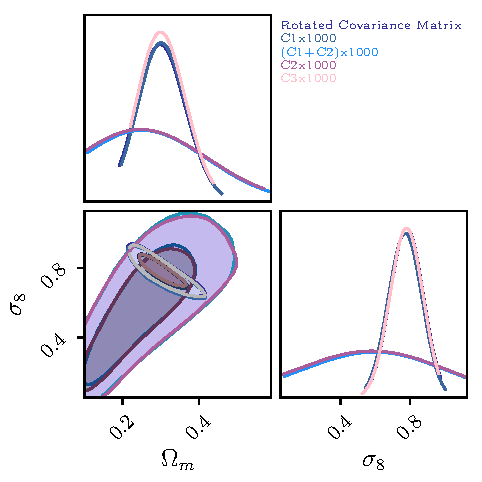
\includegraphics[width=0.9\columnwidth]{Multiply_error.pdf}
%		\caption{The upper right and lower left plots display the correlation matrix for BJ and CL respectively, while the lower right is the difference between the two. \label{fig:tolerance1000}}
%	\end{figure}
	
	
	
	%		In this section, we will introduce the methodology of tolerance testing on the covariance matrices in the new basis. We will show that after the basis transformation, we need to compare tremendously less elements from two covariance matrices.
	
	%	Generally speaking, the parameter constraints will get wider when part of the covariance matrix gets larger, because this means that the data is worse measured. In the normal basis, each data points varies with the parameter set, so the change of each element in the covariance matrix will affect the constraints. However, since we have found a basis where some of the data points change with parameter set while others do not, the elements that matters to the cosmological constraints will also shrink. To be specific, the C1 and C2 blocks in Figure~\rf{illu-trans} are the only parts that impact the parameter constraints. 
	
	%	In order to illustrate this statement, we will first perform a sanity check. We will make each of the blocks in the covariance matrices a large number and run a chain with that covariance. We run 3 tests by making
	%	1) C3,  
	%	2) C2, 
	%	3) C1 and C2,
	%	100 times of itself/themselves. In principle, we should see that the constraints for test 1 will not change but will get wider for test 2 and will totally blow up for test 3.
	
	%	Furthermore, we want to know how minor uncertainty on the informative elements of the covariance matrix will affect the cosmological constraints.